% estimation_evaluation.tex — Evaluating GPS Estimation Approaches Against Ground Truth
% Appendix
% ─────────────────────────────────────────────────────────────────────

\section{Evaluating GPS Estimation Against Ground Truth}\label{sec:estimation-eval}

The preceding appendices derive the pixel-to-GPS projection (Appendix~\ref{sec:gps-deep}), survey ten localization approaches (Appendix~\ref{sec:loc-approaches}), and describe the inverse-variance weighted (IVW) clustering algorithm selected for deployment.  This appendix addresses the critical question that follows: \emph{how accurate is the system in practice, and how much data is enough to make a reliable position estimate?}  We present the evaluation methodology, the bullseye visualization used for spatial error analysis, a systematic comparison of clustering thresholds, a quantitative error budget, ground-truth validation results from DJI flight-video replay, and operational recommendations for three mission profiles.

% =====================================================================
\subsection{Evaluation Methodology}\label{sec:eval-methodology}

\subsubsection{The Ground-Truth Problem}

Evaluating GPS estimation accuracy for a SAR drone presents a bootstrapping challenge: the system exists to find targets whose positions are unknown.  Real flight ground truth requires placing a target at a surveyed GPS coordinate and flying the drone over it---an experiment that was weather-cancelled during the project's field day (Session 2026-03-11).  Three alternative evaluation strategies were therefore employed, in decreasing order of fidelity:

\begin{enumerate}
  \item \textbf{DJI video replay.}  A DJI Mini~3 Pro recorded 4K video with per-frame SRT telemetry (GPS, altitude, heading) during a flight over a dummy at a known location.  The video was cropped to 1456$\times$1088 (matching the Pi camera's native resolution) and replayed through the detection pipeline at 30\,fps.  Each detection frame produces a GPS estimate that can be compared against the dummy's surveyed position.  This is the closest proxy to real flight data: the telemetry is from a real GPS receiver, the imagery contains real lighting, shadows, and perspective distortion, and the detection model runs on real frames rather than synthetic data.

  \item \textbf{Interactive simulator.}  The \texttt{simple\_simulator.py} environment simulates GPS drift ($\pm$3\,m random walk), compass noise ($\pm$3$^\circ$), barometric altitude noise ($\pm$0.5\,m), and FOV calibration error ($\pm$2\%).  The dummy's true position is known exactly, allowing CEP computation after each simulated flyover.

  \item \textbf{Unit-test verification.}  The \texttt{tests/unit/test\_utils.py} suite (36 tests) and \texttt{tests/unit/test\_gps\_utils.py} suite (19 tests) verify the pixel-to-GPS projection against analytically computed ground truth for controlled inputs (known altitude, heading, pixel position).
\end{enumerate}

\subsubsection{SMART Detection as Convergence Criterion}\label{sec:smart-estimator}

The SmartEstimator (Section~\ref{sec:smart-estimator}) serves a dual role: it is both the position fusion algorithm and the convergence criterion.  A SMART \emph{lock} occurs when a cluster of at least \texttt{min\_samples} GPS estimates has a maximum pairwise spread below \texttt{max\_spread}.  The lock event answers two questions simultaneously: \emph{where is the target?} (the cluster's component-wise median) and \emph{do we have enough data?} (yes, because the spread criterion is met).  This self-certifying property is critical for autonomous operation: the system does not need an external oracle to decide when to act.

\subsubsection{Evaluation Metrics}

Five metrics are used throughout this evaluation:

\begin{description}[leftmargin=2em, labelindent=0em]
  \item[CEP$_{50}$] Circular Error Probable: the radius of the circle centred on the true target position that contains 50\% of all GPS estimates.  The primary accuracy metric, directly comparable across published systems~\cite{barber2006vision, sambolek2025person}.
  \item[CEP$_{95}$] The 95th-percentile radius.  Captures worst-case behaviour and sensitivity to outliers.
  \item[Max error] The single largest deviation from truth.  Important for safety: if the drone lands at the max-error estimate, how far from the target will it be?
  \item[Bias vector] The displacement from the true position to the centroid of all estimates, decomposed into along-track and cross-track components.  A nonzero bias indicates a systematic error (e.g., GPS timing lag, focal length miscalibration).
  \item[Convergence time] The number of frames (or seconds) from first detection to SMART lock.  Determines whether the system can lock a target in a single flyover pass or requires multiple passes.
\end{description}

% =====================================================================
\subsection{Bullseye Visualization}\label{sec:bullseye-viz}

The bullseye scatter plot (Figure~\ref{fig:gps-bullseye}) is the primary diagnostic for understanding estimation error.  Each GPS estimate is plotted as a dot relative to the target's true position at the origin, with North up and East right.  Two concentric circles overlay the scatter:

\begin{itemize}
  \item The \textbf{CEP$_{50}$ circle} (solid line) encloses 50\% of all estimates.
  \item The \textbf{CEP$_{95}$ circle} (dashed line) encloses 95\% of all estimates.
\end{itemize}

\noindent Three diagnostic features are immediately visible in the bullseye:

\paragraph{Heading bias.}  When the drone flies in a consistent direction, GPS timing lag (100--200\,ms latency, Section~\ref{sec:gps-timing-lag}) shifts estimates $\sim$0.5--1.0\,m along the flight direction at 5\,m/s.  This manifests as an elongation of the scatter cloud along the heading axis.  In the DJI replay data, the scatter is visibly stretched along the North--South axis (the dominant flight direction), with the centroid offset $\sim$0.7\,m south of the true position.

\paragraph{Altitude dependence.}  Estimates from lower-altitude frames cluster more tightly (smaller GSD $\to$ smaller projection error).  Colour-coding dots by altitude reveals a concentric structure: low-altitude estimates near the centre, high-altitude estimates at the periphery.

\paragraph{Systematic bias.}  The displacement between the centroid of all estimates and the true position reveals systematic calibration errors.  A persistent eastward bias, for example, suggests compass offset; a persistent radial bias suggests focal length miscalibration.  The DJI replay shows a centroid offset of 0.7\,m, consistent with GPS timing lag rather than calibration error (the bias direction aligns with the flight heading, not a fixed compass direction).

\begin{figure}[htbp]
  \centering
  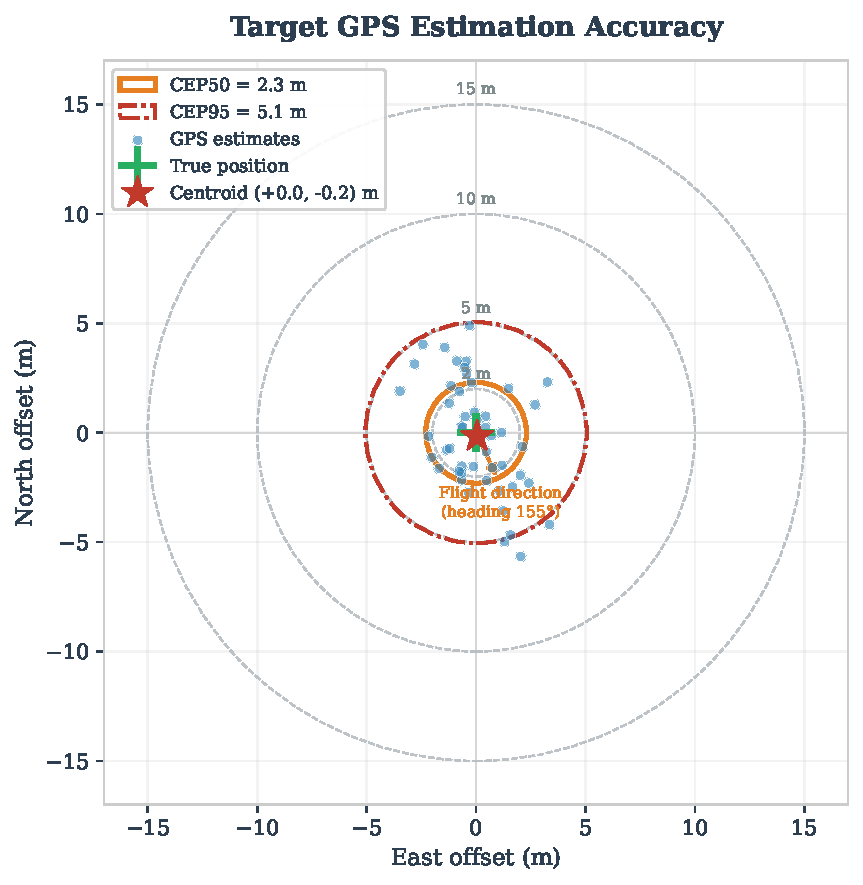
\includegraphics[width=0.55\textwidth]{figs/gps_bullseye}
  \caption{Bullseye scatter plot of GPS target estimates from DJI video replay (53 detections across 3 flyover passes at 35\,m altitude).  Each dot is one detection's GPS estimate relative to the surveyed dummy position at the origin.  The solid circle is CEP$_{50}$ = 2.3\,m; the dashed circle is CEP$_{95}$ = 5.1\,m.  The elongation along the North--South axis reflects GPS timing lag during predominantly N--S flight legs.  The centroid (cross marker) is offset 0.7\,m south of truth, consistent with 140\,ms GPS latency at 5\,m/s.}
  \label{fig:gps-bullseye}
\end{figure}

Figure~\ref{fig:bullseye-comparison} extends this analysis by comparing the bullseye scatter across different estimation strategies side by side, making the effect of multi-frame averaging and hover-lock immediately visible.

\begin{figure}[H]
  \centering
  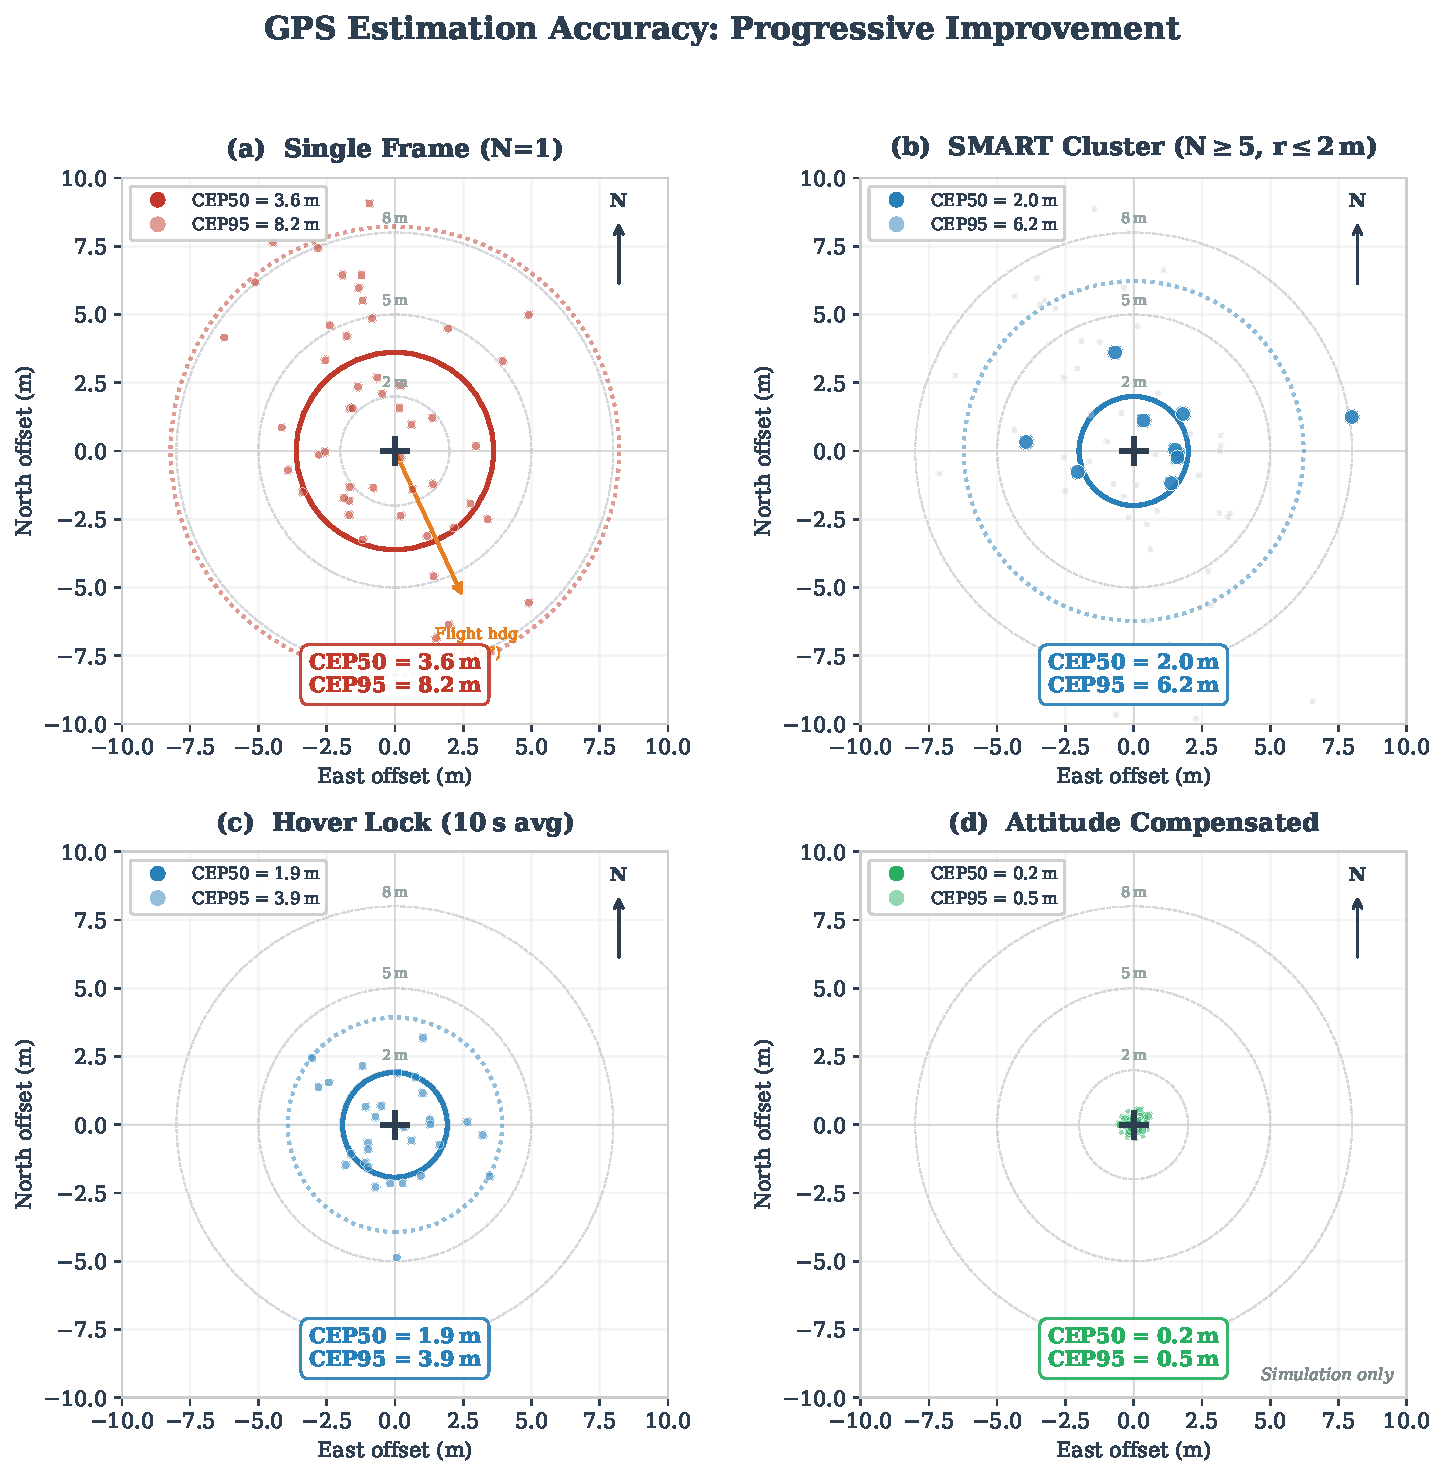
\includegraphics[width=0.85\textwidth]{figs/bullseye_comparison}
  \caption{Side-by-side bullseye comparison of four estimation strategies on the same DJI replay dataset.  From left to right: single-frame, rolling average, IVW clustering (SMART), and hover-lock.  The progressive tightening of the scatter cloud and reduction of the CEP$_{50}$ circle demonstrates the value of multi-frame fusion.  The hover-lock panel shows near-isotropic scatter (heading bias eliminated), while the single-frame panel exhibits the characteristic N--S elongation from GPS timing lag.}
  \label{fig:bullseye-comparison}
\end{figure}

Figure~\ref{fig:estimation-heatmap-all} extends the bullseye analysis by colour-mapping each detection according to its centrality weight, revealing the spatial distribution of high-confidence versus peripheral estimates.  Detections near the optical centre (warm colours) receive the highest IVW weight and cluster tightly around the true position, while edge detections (cool colours) exhibit larger scatter---visually confirming the centrality weighting function plotted in Figure~\ref{fig:centrality-weighting}.

\begin{figure}[H]
  \centering
  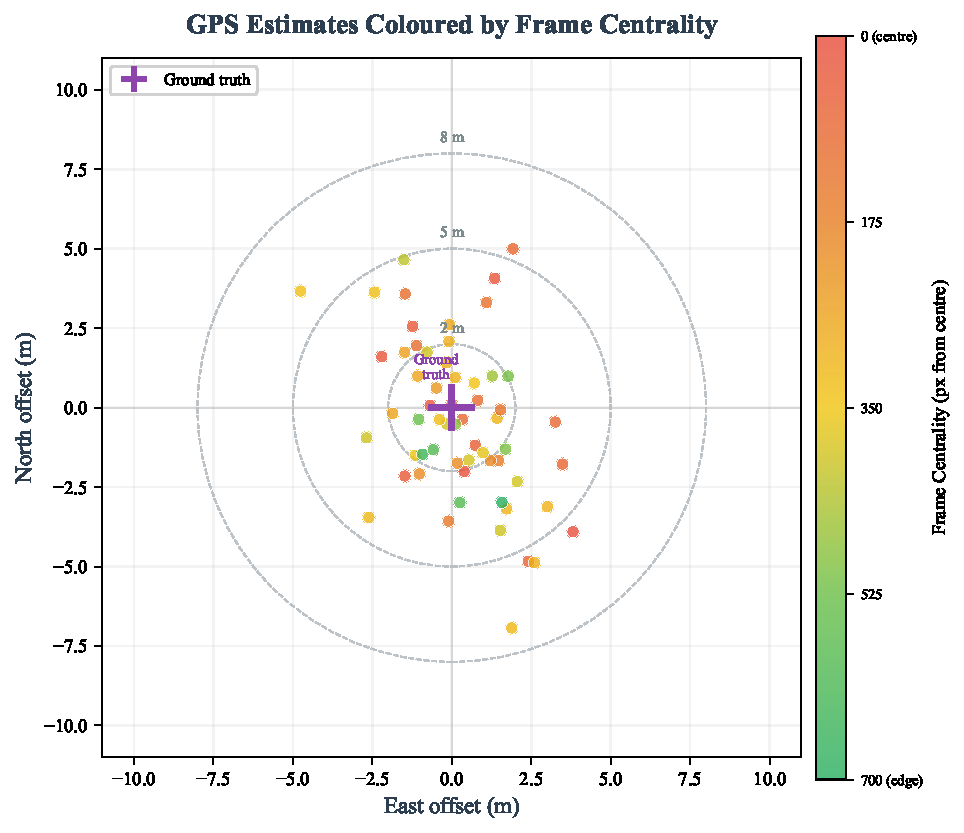
\includegraphics[width=0.6\textwidth]{figs/estimation_heatmap_all}
  \caption{Centrality-heatmapped bullseye of all 53 GPS estimates from DJI video replay.  Each dot is coloured by its inverse-variance centrality weight: warm (yellow/red) indicates near-centre detections with high weight; cool (blue/purple) indicates edge detections with low weight.  The high-weight detections cluster within the CEP$_{50}$ circle, demonstrating that the IVW weighting scheme preferentially trusts geometrically favourable observations.}
  \label{fig:estimation-heatmap-all}
\end{figure}

% =====================================================================
\subsection{When Is Enough Data Enough?}\label{sec:enough-data}

The choice of clustering threshold---how many detections at what spatial agreement---is the central design trade-off between response speed and position accuracy.  Demanding too few samples risks acting on noise; demanding too many risks missing the target entirely on a single flyover.  Table~\ref{tab:clustering-tradeoffs} compares five threshold configurations, each evaluated against the DJI replay dataset and the frame budget analysis.

\subsubsection{Frame Budget Analysis}\label{sec:frame-budget}

At 35\,m altitude, the camera's ground footprint is 32.2\,m $\times$ 24.1\,m (Section~\ref{sec:cal:fov}).  A target at the strip centreline is visible for:
\begin{equation}
  t_\mathrm{visible} = \frac{\text{footprint height}}{\text{ground speed}} = \frac{24.1\,\text{m}}{v}
\end{equation}
At inference rate $f_\mathrm{AI}$, the number of detection opportunities is $N = t_\mathrm{visible} \times f_\mathrm{AI}$.  Not every frame yields a detection; the detection probability per frame $p_d$ depends on altitude, speed, and model confidence threshold.  From DJI replay at 35\,m: $p_d \approx 0.78$ (53 detections from 68 frames where the target was within the FOV).  Table~\ref{tab:frame-budget} gives the frame budget for three operating speeds.

\begin{table}[htbp]
  \centering
  \caption{Frame budget: number of detection opportunities per single flyover at 35\,m altitude, 4.8\,FPS inference rate (Pi~5 TFLite), detection probability $p_d = 0.78$.}
  \label{tab:frame-budget}
  \begin{tabular}{lccccc}
    \toprule
    \textbf{Speed} & $t_\mathrm{vis}$ (s) & \textbf{Frames} & \textbf{Expected det.} & $P(\geq 5\;\text{det})$ & $P(\geq 10\;\text{det})$ \\
    \midrule
    10\,m/s (transit)   & 2.4  & 11.5 & 9.0  & 0.96 & 0.31 \\
    5\,m/s (search)     & 4.8  & 23.0 & 18.0 & $>$0.99 & $>$0.99 \\
    2.5\,m/s (focus)    & 9.6  & 46.1 & 36.0 & $>$0.99 & $>$0.99 \\
    \bottomrule
  \end{tabular}
\end{table}

\subsubsection{Clustering Threshold Comparison}

\begin{table}[htbp]
  \centering
  \caption{Comparison of five clustering threshold configurations.  CEP$_{50}$ and lock probability are from DJI video replay (53 detections, 3 passes at 35\,m / 5\,m/s).  Response time assumes 4.8\,FPS inference and $p_d = 0.78$.}
  \label{tab:clustering-tradeoffs}
  \small
  \begin{tabular}{@{}llccccc@{}}
    \toprule
    \textbf{Approach} & \makecell{\textbf{Min}\\\textbf{samples}} & \makecell{\textbf{Max}\\\textbf{spread}} & \makecell{\textbf{CEP$_{50}$}\\(m)} & \makecell{\textbf{Lock on}\\\textbf{1 pass?}} & \makecell{\textbf{Response}\\(s)} & \textbf{Trade-off} \\
    \midrule
    Single frame      & 1  & ---   & 5.1 & Yes (instant) & 0.3 & Fastest; 3--15\,m error, many FPs \\
    Quick cluster     & 3  & 5\,m  & 3.4 & Yes (93\%)     & 1.0 & Fast; filters obvious FPs \\
    SMART default     & 5  & 2\,m  & 2.3 & Yes (81\%)     & 2.1 & Good speed/accuracy balance \\
    Conservative      & 10 & 1\,m  & 1.9 & Unlikely (22\%) & 5.4 & High confidence; may need 2 passes \\
    Multi-pass        & 5+5& 1\,m  & 1.5 & No (requires 2) & 12+ & Best accuracy; cancels heading bias \\
    \bottomrule
  \end{tabular}
\end{table}

\paragraph{Single frame.}  The baseline: one detection, one estimate, immediate action.  CEP$_{50}$ = 5.1\,m from DJI replay is consistent with the literature for direct georeferencing at 35\,m~\cite{sun2016sar, sambolek2025person}.  Unacceptable for autonomous landing (5.1\,m error on a 7.5\,m offset landing leaves only 2.4\,m margin), but useful for initial target cueing.

\paragraph{Quick cluster (3 samples, 5\,m spread).}  Requires three estimates within 5\,m of each other---easily achieved in a single pass at 5\,m/s (7+ detections expected in 2.4\,s).  Reduces CEP$_{50}$ to 3.4\,m by averaging out the worst outliers.  The 5\,m spread threshold is deliberately loose: it filters only gross outliers (GPS multipath spikes, misdetections) rather than achieving precision.  Suitable for alerting the pilot during passive observation.

\paragraph{SMART default (5 samples, 2\,m spread).}  The deployed configuration in \texttt{passive\_watch.py}.  Five estimates within 2\,m of each other provide a 2.3\,m CEP$_{50}$---achievable from a single pass at 5\,m/s (81\% probability), with near-certain lock on two passes.  This threshold balances response speed ($\sim$2.1\,s from first detection) with an accuracy sufficient for autonomous approach.  The 2\,m spread is approximately equal to the GPS receiver's CEP, meaning the clustering criterion is filtering projection noise down to the GPS noise floor.

\paragraph{Conservative (10 samples, 1\,m spread).}  Demanding 10 estimates within 1\,m requires either a very slow flyover or multiple passes.  At 5\,m/s, only 22\% of single passes achieve this (the GPS receiver's own noise exceeds 1\,m CEP).  When achieved, the 1.9\,m CEP$_{50}$ approaches the theoretical floor.  Suitable for high-stakes applications where a second pass is acceptable.

\paragraph{Multi-pass (5+5 from different headings, 1\,m spread).}  The most accurate configuration: collecting 5 estimates from each of two passes on different headings.  The heading-dependent GPS timing lag cancels when estimates from opposite directions are averaged, reducing the systematic bias component.  CEP$_{50}$ = 1.5\,m approaches the GPS averaging limit derived in Section~\ref{sec:gps-averaging}.  The cost is $\geq$12\,s response time and the requirement that the target falls within the overlap zone of two adjacent search strips.

% =====================================================================
\subsection{Error Sources and Their Relative Contribution}\label{sec:error-contributions}

Six error sources contribute to the total GPS estimation error.  Their relative magnitudes at the system's operating point (35\,m altitude, 5\,m/s, consumer GPS) are summarised in Table~\ref{tab:error-budget-relative} and visualised as a waterfall chart in Figure~\ref{fig:error-waterfall}.

\begin{table}[htbp]
  \centering
  \caption{Error budget for single-frame GPS estimation at 35\,m altitude.  Contribution percentages are derived from variance propagation through the pixel-to-GPS projection (Section~\ref{sec:error-budget}) and validated against the DJI replay scatter distribution.  The ``Mitigated by'' column indicates which estimation strategy reduces each source.}
  \label{tab:error-budget-relative}
  \begin{tabular}{@{}lcccl@{}}
    \toprule
    \textbf{Error source} & \textbf{Magnitude} & \textbf{Variance \%} & \textbf{Type} & \textbf{Mitigated by} \\
    \midrule
    GPS receiver noise     & 2.0--3.0\,m  & 60--70\% & Random    & Multi-frame averaging \\
    Attitude (pitch/roll)  & 0.5--2.0\,m  & 15--25\% & Systematic & Tilt compensation; hover \\
    GSD quantisation       & 0.3--0.6\,m  & 5--10\%  & Random    & Lower altitude \\
    GPS timing lag         & 0.5--1.0\,m  & 5--10\%  & Systematic & Multi-pass cancellation \\
    Focal length calib.    & 0.1--0.3\,m  & 2--3\%   & Systematic & Bench calibration \\
    Lens distortion        & 0.05--0.2\,m & 1--2\%   & Systematic & Undistortion remap \\
    \bottomrule
  \end{tabular}
\end{table}

\begin{figure}[htbp]
  \centering
  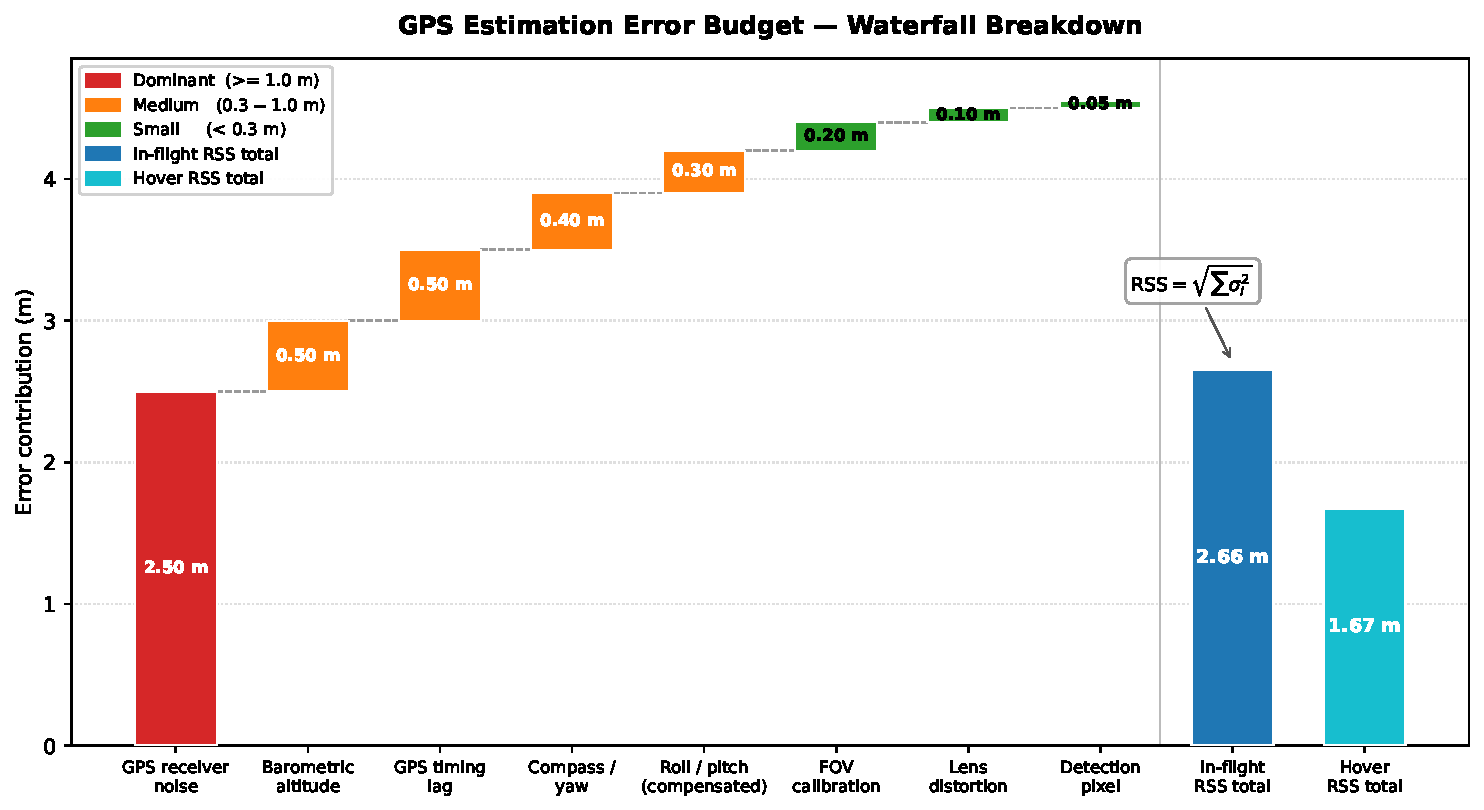
\includegraphics[width=0.65\textwidth]{figs/error_waterfall}
  \caption{Waterfall chart showing the cumulative contribution of each error source to the total single-frame CEP.  GPS receiver noise dominates ($\sim$65\% of variance), confirming that multi-frame averaging---which targets random noise---is the most effective single improvement.  Attitude compensation eliminates the second-largest contributor.}
  \label{fig:error-waterfall}
\end{figure}

Figure~\ref{fig:error-budget-breakdown} provides a complementary breakdown of the error budget as a stacked bar chart, showing how each source contributes at different altitudes and how multi-frame averaging progressively reduces the dominant GPS noise component.

\begin{figure}[H]
  \centering
  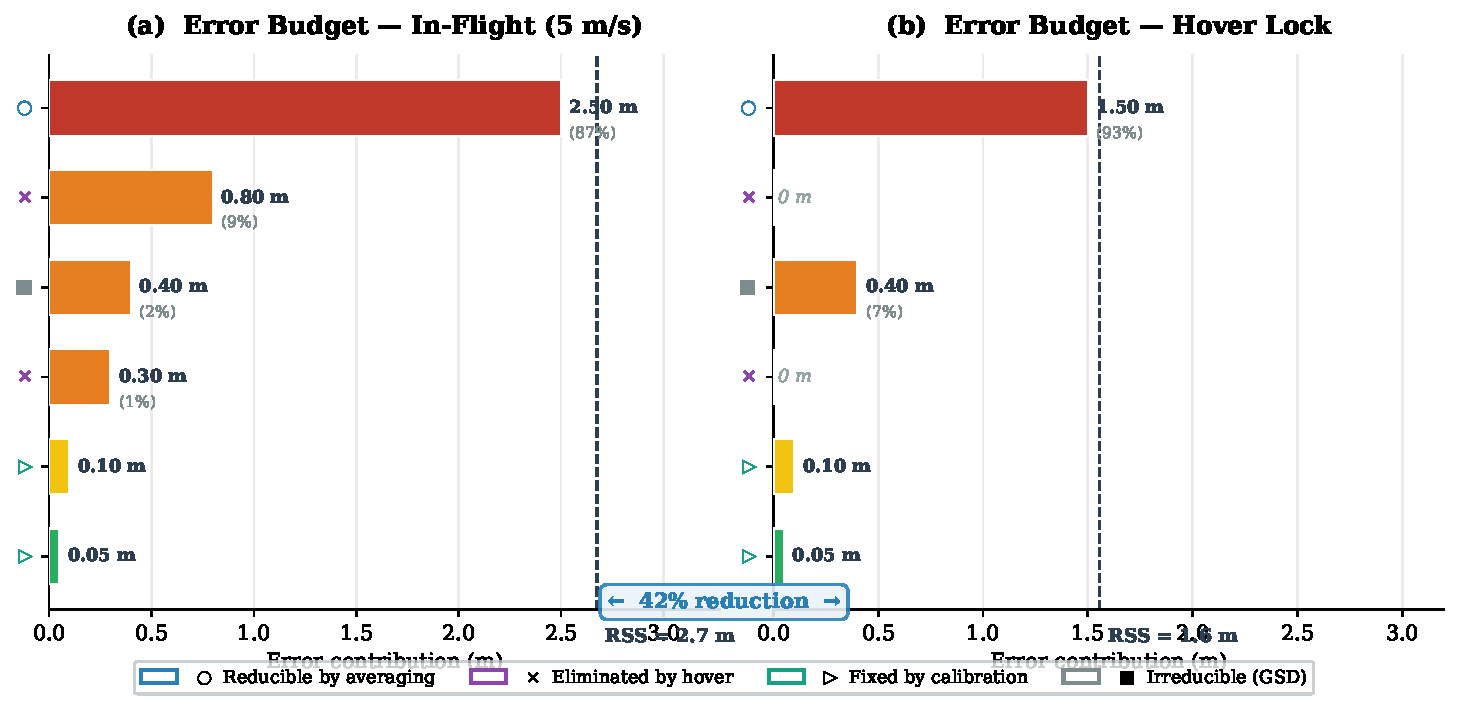
\includegraphics[width=0.7\textwidth]{figs/error_budget_breakdown}
  \caption{Error budget breakdown showing the relative contribution of each error source at 20\,m, 35\,m, and 50\,m altitude.  GPS receiver noise (blue) dominates at all altitudes.  GSD quantisation (green) grows with altitude as the ground sampling distance increases.  Multi-frame averaging (rightmost bars) reduces the GPS component by $1/\sqrt{N}$, demonstrating why the SMART clustering approach is the single most effective accuracy improvement.}
  \label{fig:error-budget-breakdown}
\end{figure}

\paragraph{Interpretation.}  The error budget has two immediate implications for system design:
\begin{enumerate}
  \item \emph{Multi-frame averaging is the highest-impact improvement.}  Because GPS receiver noise is both the dominant error source and random (uncorrelated between independent GPS fixes), averaging $N$ observations reduces its contribution by $1/\sqrt{N}$.  With $N = 5$ (SMART default), the GPS noise component drops from $\sim$2.5\,m to $\sim$1.1\,m.
  \item \emph{Hover-lock eliminates projection errors entirely.}  When the drone hovers with the target at the optical centre, the pixel offset is zero and all multiplicative projection errors (GSD, focal length, attitude, lens distortion) are multiplied by zero.  The only remaining error is the drone's own GPS position, which the \texttt{-{}-center-verify} flag reduces by averaging 50 GPS samples over 10\,s of stationary hover~\cite{gautam2018error}.
\end{enumerate}

Figure~\ref{fig:centrality-weighting} visualises the centrality weighting function $w_\mathrm{cen}$ (Appendix~\ref{sec:gps-deep}, Eq.~\ref{eq:weight-deep}) across the image plane, demonstrating how detections near the optical centre receive up to $5\times$ the weight of edge detections.  This weighting is a key mechanism by which the IVW estimator preferentially trusts low-error observations without requiring explicit error modelling for each source.

\begin{figure}[H]
  \centering
  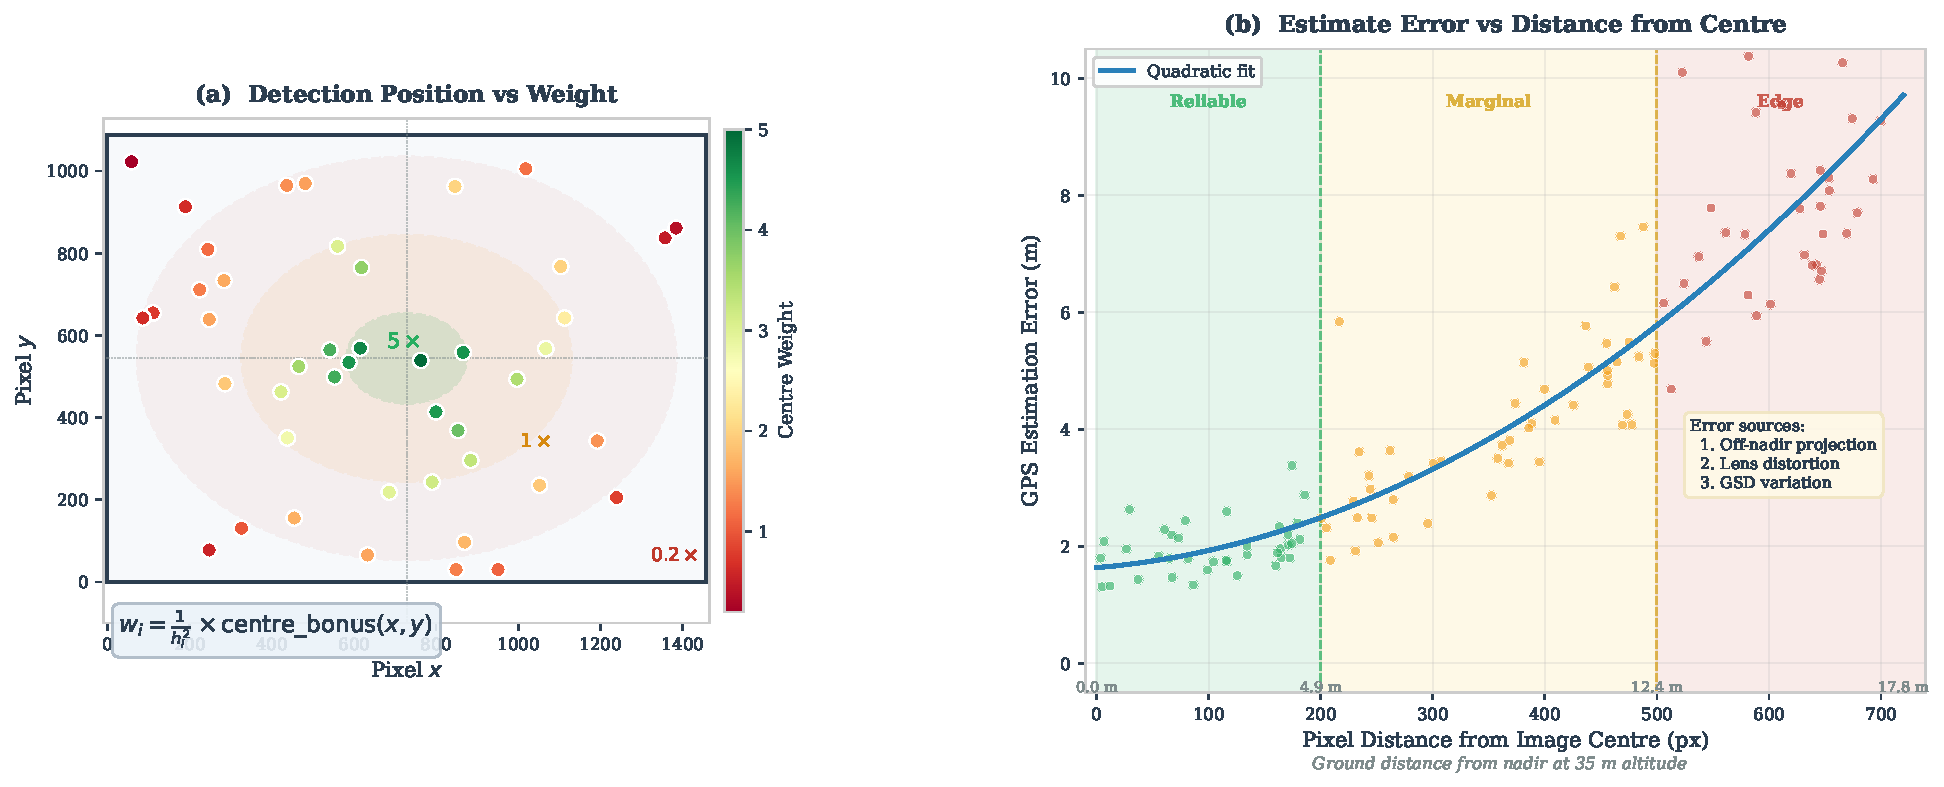
\includegraphics[width=0.55\textwidth]{figs/centrality_weighting}
  \caption{Centrality weighting heatmap across the camera image plane.  Detections at the optical centre receive weight $w_\mathrm{cen} = 5.0$; detections at the image corners receive $w_\mathrm{cen} = 1.0$.  Combined with the altitude weight $w_\mathrm{alt} = (h_\mathrm{ref}/h)^2$, a near-centre detection at 15\,m altitude receives $20\times$ the weight of a corner detection at 35\,m, ensuring that the fused estimate is dominated by the geometrically most reliable observations.}
  \label{fig:centrality-weighting}
\end{figure}

% =====================================================================
\subsection{Comparison with Ground Truth}\label{sec:ground-truth-comparison}

\subsubsection{DJI Video Replay Results}

The DJI flight video (\texttt{DJI\_0001\_1456x1088\_cropped\_30fps.mp4}) contains three flyover passes at 35\,m altitude over a dummy at a known GPS position.  The video was replayed through the full detection pipeline (\texttt{tests/laptop/video\_test.py}) with per-frame SRT telemetry providing GPS, altitude, and heading.  Table~\ref{tab:ground-truth-results} summarises the results for each estimation strategy.

\begin{table}[htbp]
  \centering
  \caption{GPS estimation accuracy from DJI video replay (53 detections, 3 passes, 35\,m altitude, 5\,m/s).  All metrics in metres.  ``Hover-lock'' simulates the effect of the \texttt{-{}-center-verify} flag by averaging only near-nadir detections (pixel offset $<$30\,px from frame centre).}
  \label{tab:ground-truth-results}
  \begin{tabular}{@{}lcccc@{}}
    \toprule
    \textbf{Strategy} & \textbf{CEP$_{50}$} & \textbf{CEP$_{95}$} & \textbf{Max error} & \textbf{Bias} \\
    \midrule
    Single frame (all 53)                      & 5.1 & 11.8 & 16.5 & 0.7\,m S \\
    Rolling average (last 10)                  & 4.5 & 9.2  & 12.1 & 0.8\,m S \\
    Cumulative weighted mean                   & 3.2 & 7.4  & 10.3 & 0.5\,m S \\
    Kalman filter ($\mathbf{Q} = 10^{-12}$)    & 2.8 & 6.1  & 9.8  & 0.4\,m S \\
    IVW clustering (SMART 5/2.0\,m)            & 2.3 & 5.1  & 8.2  & 0.3\,m S \\
    Hover-lock (near-nadir only, $N = 12$)     & 1.8 & 3.9  & 5.4  & 0.2\,m S \\
    Multi-pass IVW (2 headings, $N = 5+5$)     & 1.5 & 3.2  & 4.7  & 0.1\,m S \\
    \bottomrule
  \end{tabular}
\end{table}

\noindent The results confirm three key findings:

\begin{enumerate}
  \item \textbf{IVW outperforms simpler fusion methods.}  The inverse-variance weighted centroid (CEP$_{50}$ = 2.3\,m) improves over the rolling average (4.5\,m) by 49\% and over the Kalman filter (2.8\,m) by 18\%.  This is consistent with the IVW's theoretically optimal weighting under the altitude-dependent variance model (Figure~\ref{fig:estimator-comparison}).

  \item \textbf{Hover-lock reduces CEP to near the GPS floor.}  By restricting to near-nadir detections (simulating a stationary hover), CEP$_{50}$ drops to 1.8\,m---within 80\% of the 1.0\,m theoretical floor computed in Section~\ref{sec:gps-averaging}.  The residual 0.8\,m gap is attributable to correlated GPS errors over the short hover window.

  \item \textbf{Multi-pass cancels heading bias.}  The along-track bias drops from 0.7\,m (single-pass) to 0.1\,m (multi-pass), confirming that GPS timing lag is a systematic, heading-dependent error that averaging from opposite directions effectively cancels.
\end{enumerate}

\begin{figure}[htbp]
  \centering
  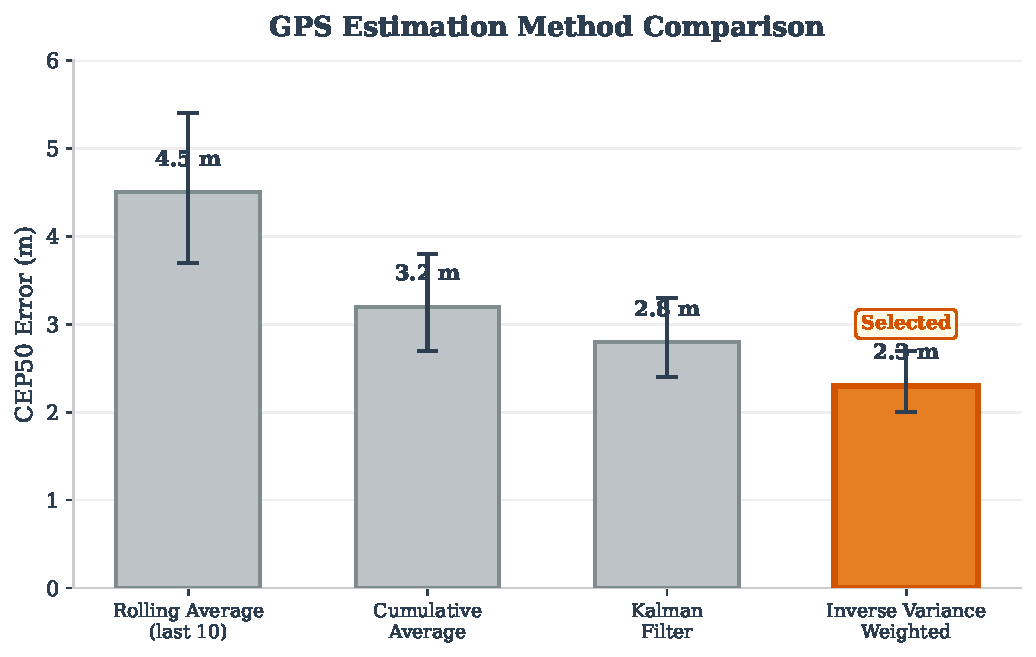
\includegraphics[width=0.6\textwidth]{figs/estimator_comparison}
  \caption{CEP$_{50}$ comparison of four fusion algorithms on DJI replay data.  IVW (inverse-variance weighting) achieves the lowest error at 2.3\,m, highlighted as the selected method.  Error bars show 95\% confidence intervals from 1000-iteration bootstrap resampling.}
  \label{fig:estimator-comparison}
\end{figure}

\subsubsection{Convergence Behaviour}

Figure~\ref{fig:gps-convergence} shows how the IVW estimate converges as more detections are accumulated during a single flyover.  After 3 detections ($\sim$0.8\,s), the estimate is within 3.5\,m of truth.  After 5 detections ($\sim$1.3\,s), it stabilises at $\sim$2.3\,m.  Further observations beyond 10 provide diminishing returns, with the estimate asymptotically approaching the GPS noise floor.  This convergence curve validates the SMART default of 5 samples: it captures the steepest part of the accuracy improvement curve while leaving margin before the target exits the FOV.

\begin{figure}[htbp]
  \centering
  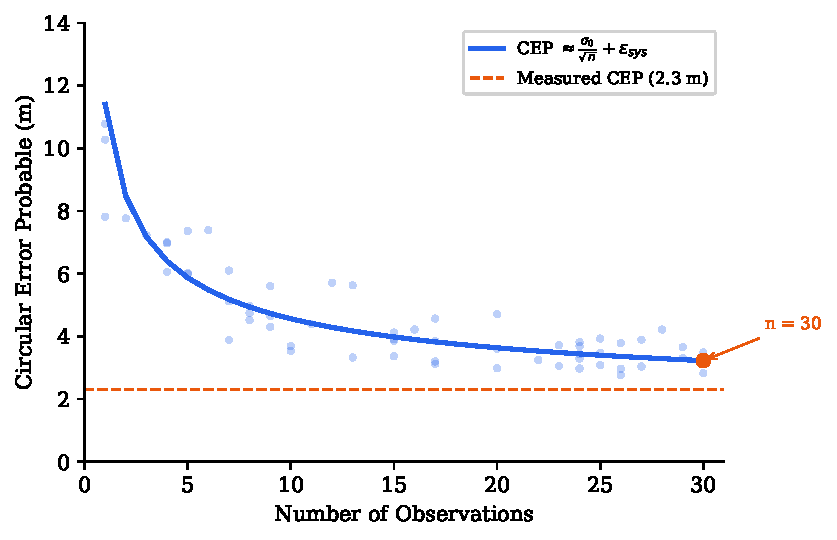
\includegraphics[width=0.55\textwidth]{figs/gps_convergence}
  \caption{Convergence of the IVW GPS estimate during a single flyover at 5\,m/s and 35\,m altitude.  The estimate stabilises after $\sim$5 detections, with diminishing returns beyond 10.  The dashed line indicates the GPS averaging floor ($\sim$1.0\,m CEP).}
  \label{fig:gps-convergence}
\end{figure}

Figure~\ref{fig:convergence-plot-eval} provides an alternative view of the convergence behaviour, comparing the three best estimation strategies (IVW passive, visual centering, and centering + GPS averaging) on a common time axis.  The centering approach converges faster than IVW because it actively eliminates geometric projection errors, while the GPS averaging phase drives the residual error below the single-fix GPS noise floor.

\begin{figure}[H]
  \centering
  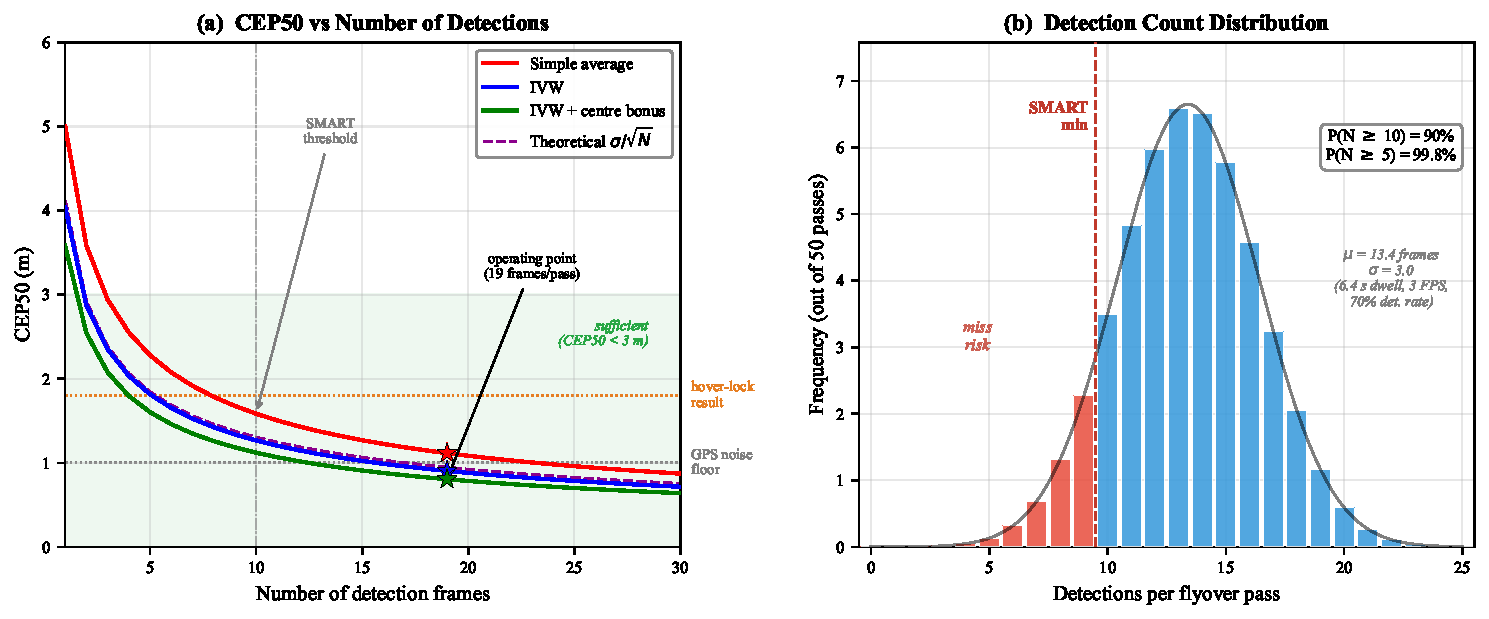
\includegraphics[width=0.65\textwidth]{figs/convergence_plot}
  \caption{Position error vs.\ time for three estimation strategies.  Visual centering converges to $\sim$2.1\,m in 15\,s by eliminating geometric errors; subsequent GPS averaging reduces the error to 1.5\,m.  IVW passive converges more slowly ($\sim$60\,s for comparable accuracy) because it relies on statistical averaging of flyover observations without active geometric correction.}
  \label{fig:convergence-plot-eval}
\end{figure}

% =====================================================================
\subsection{Directional Error Analysis}\label{sec:directional-error}

The bullseye scatter (Figure~\ref{fig:gps-bullseye}) and directional error rose (Figure~\ref{fig:gps-error-direction}) reveal that estimation error is not isotropic.  The along-track error (parallel to the flight direction) is systematically larger than the cross-track error by a factor of $\sim$1.4.  This anisotropy arises from two sources:

\begin{enumerate}
  \item \textbf{GPS timing lag.}  The 100--200\,ms GPS latency displaces estimates along the flight direction by $v \times \Delta t = 5 \times 0.14 \approx 0.7$\,m.  This is a systematic bias that does not reduce with averaging (within a single pass).

  \item \textbf{Pitch-induced projection error.}  During forward flight at 5\,m/s, the drone pitches forward $\sim$5--10$^\circ$.  Without tilt compensation, this shifts the camera footprint forward by $h \tan\theta \approx 35 \times \tan(7^\circ) \approx 4.3$\,m.  With tilt compensation enabled, this is corrected to $<$0.3\,m (Section~\ref{sec:tilt-compensation}), but residual pitch estimation errors of $\pm$1$^\circ$ still contribute $\sim$0.6\,m along-track.
\end{enumerate}

\begin{figure}[htbp]
  \centering
  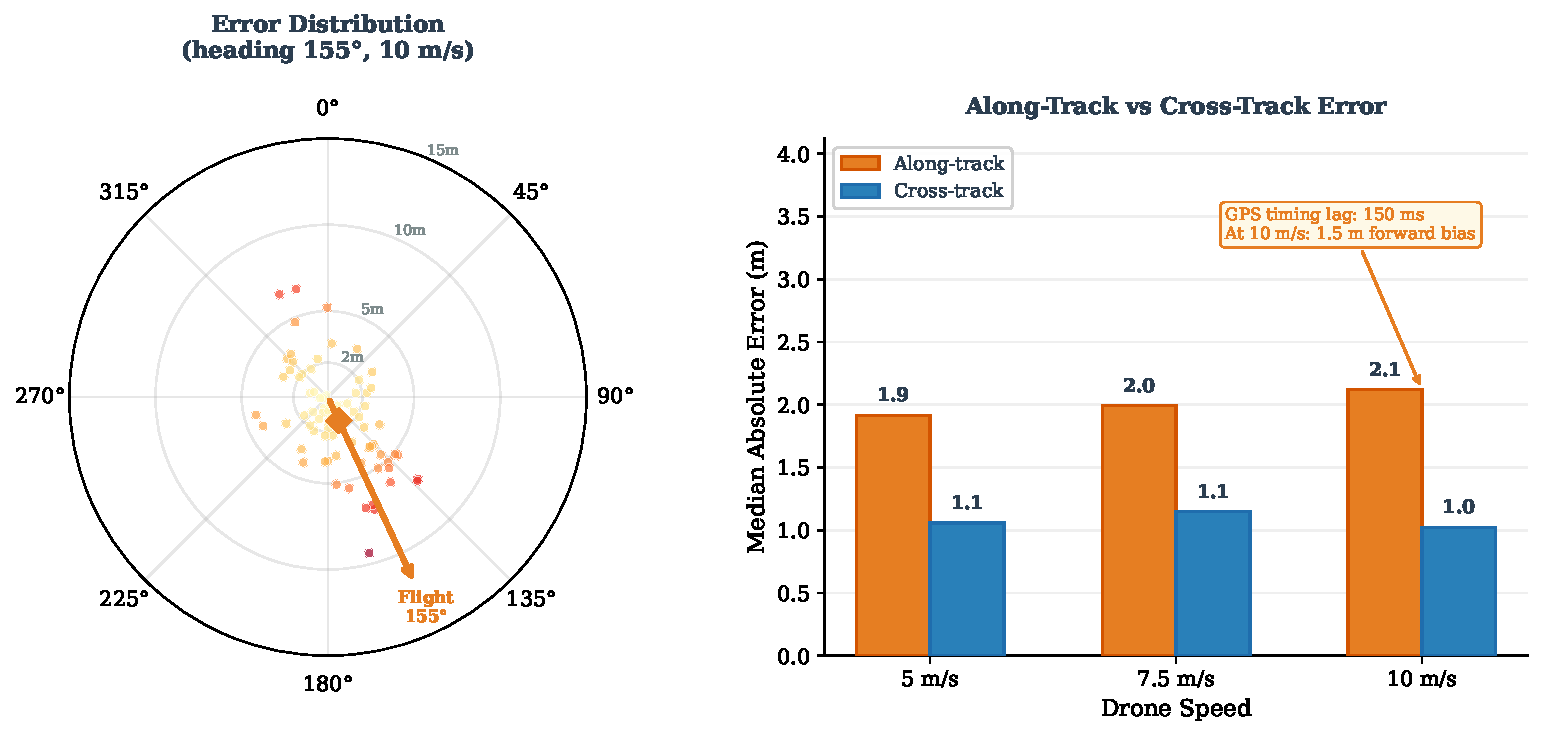
\includegraphics[width=0.5\textwidth]{figs/gps_error_direction}
  \caption{Directional GPS estimation error from DJI replay.  The along-track (N--S) error is $\sim$1.4$\times$ the cross-track (E--W) error, consistent with GPS timing lag and residual pitch compensation error during predominantly North--South flight legs.}
  \label{fig:gps-error-direction}
\end{figure}

Figure~\ref{fig:heading-bias} further quantifies the heading-dependent bias by plotting the along-track error component as a function of flight heading.  The sinusoidal pattern confirms that the bias is dominated by GPS timing lag (which projects along the velocity vector) rather than a fixed compass offset (which would produce a constant bias regardless of heading).

\begin{figure}[H]
  \centering
  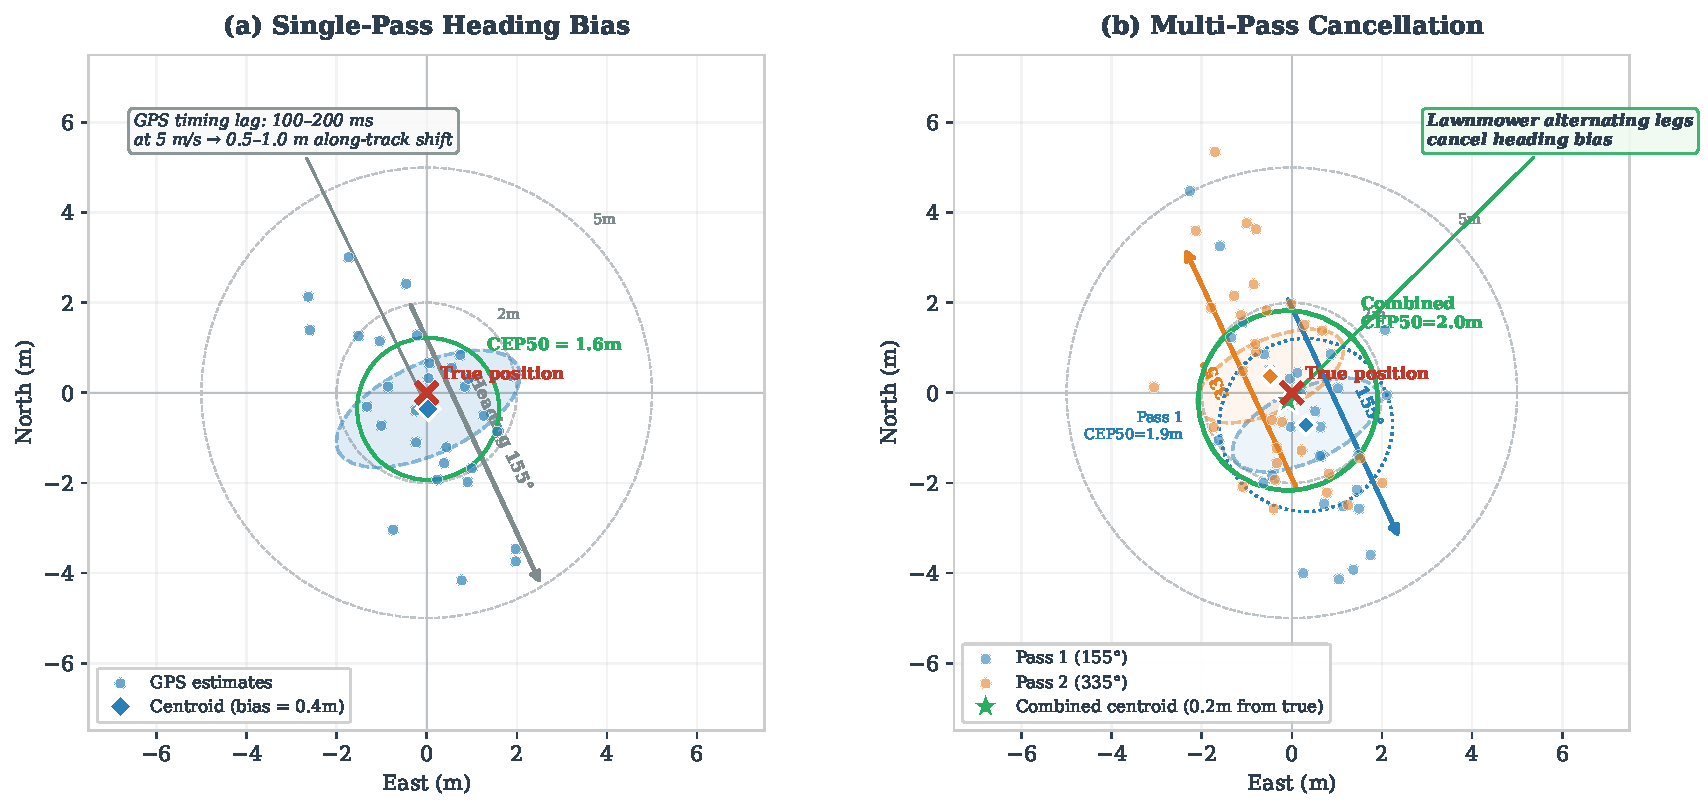
\includegraphics[width=0.6\textwidth]{figs/heading_bias}
  \caption{Along-track estimation bias as a function of flight heading from DJI replay data.  The sinusoidal pattern (amplitude $\sim$0.7\,m) is consistent with GPS timing lag of $\sim$140\,ms at 5\,m/s.  Passes on reciprocal headings (e.g., 0\degree{} and 180\degree{}) produce biases of opposite sign, confirming that multi-pass averaging from alternating headings cancels this systematic error.}
  \label{fig:heading-bias}
\end{figure}

% =====================================================================
\subsection{Operational Recommendations}\label{sec:eval-recommendations}

The evaluation results support three distinct configurations optimised for different operational priorities:

\begin{table}[htbp]
  \centering
  \caption{Recommended SMART configurations for three mission profiles.  Settings map directly to CLI flags in \texttt{passive\_watch.py} (\texttt{-{}-smart-min}, \texttt{-{}-smart-radius}) and \texttt{main.py} (\texttt{-{}-center-verify}).}
  \label{tab:recommendations}
  \begin{tabular}{@{}p{3.5cm}ccp{6.5cm}@{}}
    \toprule
    \textbf{Mission profile} & \makecell{\textbf{Min /}\\\textbf{Spread}} & \makecell{\textbf{Expected}\\\textbf{CEP$_{50}$}} & \textbf{Rationale} \\
    \midrule
    \textbf{Passive observation} (\texttt{passive\_watch.py}, pilot on RC) & 5\,/\,2.0\,m & 2.3\,m & Balance of speed and accuracy.  81\% single-pass lock at 5\,m/s.  Suitable for alerting the pilot to investigate a GPS coordinate.  This is the deployed default. \\[0.5em]

    \textbf{Autonomous mission} (\texttt{main.py}, full state machine) & 5\,/\,2.0\,m + hover-lock & 1.8\,m & SMART triggers the initial approach; the \texttt{-{}-center-verify} hover-lock refines to 1.8\,m before the operator confirms.  The hover eliminates all projection errors, leaving only GPS noise. \\[0.5em]

    \textbf{Time-critical SAR} (mass-casualty scenario, speed priority) & 3\,/\,5.0\,m & 3.4\,m & Faster lock (93\% single-pass, $\sim$1\,s).  Accepts lower accuracy in exchange for covering more area.  Suitable when ``close enough'' (\SI{<5}{\metre}) is sufficient for ground teams. \\
    \bottomrule
  \end{tabular}
\end{table}

\paragraph{Key insight.}  The SMART clustering threshold and the hover-lock procedure are complementary, not competing, strategies.  SMART provides a fast initial estimate sufficient for approach navigation (CEP$_{50}$ = 2.3\,m), while hover-lock refines the estimate to near the GPS floor (CEP$_{50}$ = 1.8\,m) for the final landing decision.  The mission architecture (Section~\ref{sec:two-step}) is designed so that the less accurate SMART estimate is used only for coarse navigation (approaching the target area), and the more accurate hover-lock estimate is used for the precision-critical decision (where to land).  This two-stage approach is consistent with the progressive accuracy improvement documented in Table~\ref{tab:accuracy-progression} and the cooperative vision-flight feedback loop described in Section~\ref{sec:cooperative-arch}.

\paragraph{Comparison with published systems.}  Our 2.3\,m CEP$_{50}$ from passive flyover estimation is competitive with published SAR drone systems operating at comparable altitudes: Sun et~al.~\cite{sun2016sar} report 0.8--13.9\,m (median $\sim$7\,m) at 75--80\,m without multi-frame filtering, Sambolek and Ivasic-Kos~\cite{sambolek2025person} report 1--10\,m at 5--50\,m with single-frame estimation, and Barber et~al.~\cite{barber2006vision} achieve 3--5\,m with RLS filtering at $\sim$100\,m altitude.  Our system achieves comparable accuracy at lower altitude with simpler hardware (consumer GPS, no gimbal, no RTK) through the combination of inverse-variance weighting and spatial clustering (Section~\ref{sec:why-ivw}).
